\documentclass{article}
\usepackage{fixltx2e}
\usepackage[utf8]{inputenc}
\usepackage{graphicx}
\usepackage{sidecap}
\usepackage{fancyhdr}
\usepackage[margin=1.5in]{geometry}
\setlength{\headheight}{21pt}

\begin{document}

% Titelsida -----------------------------
\begin{titlepage}
\begin{center}

% Upper part of the page. The '~' is needed because \\
% only works if a paragraph has started.

\textsc{\LARGE Link{\"o}pings Universitet}\\[1.5cm]


% Title
{ \huge \bfseries Modellbaserad reglering av dubbeltankar \\[0.4cm] }

% Author and supervisor
\large
\emph{Av:}\\
Hans-Filip \textsc{Elo} och Niklas \textsc{Ericson}

\vfill

% Bottom of the page
{\large \today}

\end{center}
\end{titlepage}

% Slut på titelsida. ---------------------

% Innehåll ------------------------------

%header ---------------------------------
\pagestyle{fancy}

\fancyhead{} % clear all header fields
\fancyhead[L]{TSRT12\slshape}
\fancyhead[R]{\today \slshape}

\fancyfoot{} % clear all footer fields
\fancyfoot[L,R]{\thepage}
\fancyfoot[L]{Modellbaserad reglering av dubbeltankar}

%slut på header ---------------------------------


\section{Inledning}
En överföringsfunktions egenskaper så som stigtid, översläng och felmarginal går att påverka genom att multiplicera funktionen med en deriverande, F\textsubscript{lead}, och en integrerande, F\textsubscript{lag}, funktion. En laboration med ett dubbeltanksystem har genomförts för att applicera teorin i verkligheten.

\subsection{Syfte}
Syftet med laborationen var att utifrån en given överföringsfunktion, förändra systemets egenskaper med hjälp av Lead och Lag funktioner.

\section{Metod}
Laborationen bestod av 2 delar. Första delen bestod av att ta fram två okända konstanter, {\itshape T} och {\itshape K}\textsubscript{dubbel} och den andra delen bestod i att ta fram en F\textsubscript{lead} och en F\textsubscript{lag} funktion som gav önskade egenskaper på systemet.

\subsection{Framtagning av T och K\textsubscript{dubbel}}
I föreberedelseuppgifterna till laboration visades det att tidskonstanten, {\itshape T} fås av den tid det tar för stegsvaret att nå 63\% av slutvärdet. 

\subsection{Förändring av systemets egenskaper}


\begin{figure}[ht!]
\centering
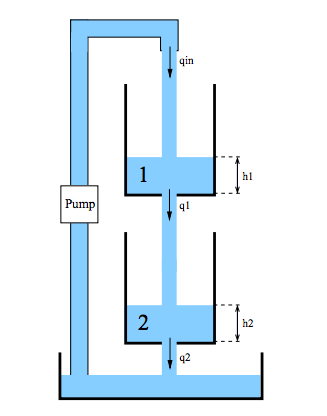
\includegraphics[width=70mm]{System.png}
\caption{Visualisering av labuppkopplingen}
\label{overflow}
\end{figure}

\subsection{Materiel}

\section{Resultat}

\begin{figure}[ht!]
\centering
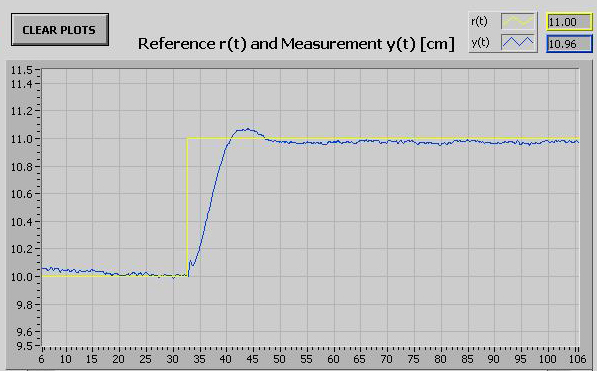
\includegraphics[width=90mm]{Test1_cut.jpg}
\caption{Stegsvaret efter kompensering med F\textsubscript{lead} och F\textsubscript{lag}.}
\label{overflow}
\end{figure}


\section{Slutsats}

\end{document}